\iffalse METRICS
- Numerical stability of different conformal mapping methods
- Boundary discretization requirements (how smooth does $\gamma$ need to be?)
- Mesh quality preservation - how does the mapping affect triangle quality?
- Computational complexity
- Input and output formats
- https://www.desmos.com/calculator/g9asjc6xph
\fi
\section{Existing Methods}
This chapter aims to give an overview and compare some existing methods in terms of input/output format, requirements on the boundary or shape of the regions, computational complexity, numerical stability and mesh quality preservation/ accuracy. The list is non-exhaustive but covers some of the most well-known and widely used methods.

We start with an overview of the methods covered and how to choose between them depending on the application before explaining each of them in more detail.
% THIS SHOULD GIVE A COMPREHENSIBLE OVERVIEW OF POTENTIAL METHODS AND HOW TO CHOOSE THEM
\begin{center}
    \red{maybe change to first boundary smooth then BIE, if not smooth then at least piecewise continuous then SCE, else if not well-behaved IDK}
\begin{tikzpicture}[node distance=1cm]

\node (BVP) {BVP};

\node (Q_poly) [below=of BVP] {$\Omega$ a polygon?};

\node (SCE) [right=of Q_poly] {Schwarz-Christoffel};

\node (Q_BIE) [below=of Q_poly] {Reformulate as BIE?};

\node (Q_star) [below=of Q_BIE] {$\Omega$ star-shaped?};

\node (theo) [below=of Q_star] {Theodorsen's Equation};

\node (BIE) [right=of Q_star] {General BIE Methods};
\node (kerz) [below=of BIE] {Kerzman-Stein};
\node (neu) [below left=of kerz, xshift=1cm] {Neumann Kernel};
\node (symm) [below right=of BIE] {Symm's Equation*};
\node (amano) [below=of symm] {Amano's Method};

\node (other) [right=of Q_BIE] {Other Method Families};
\node (zip) [above right=of other] {Zipper};
\node (berg) [right=of other] {Bergman Kernel};
\node (AP) [below right=of other] {Alternating Projections};

\draw [->] (BVP) -- (Q_poly);

\draw [->] (Q_poly) -- (SCE) 
    node [midway, above] {Yes};
\draw [->] (Q_poly) -- (Q_BIE) 
    node [midway, left] {No};

\draw [->] (Q_BIE) -- (Q_star) 
    node [midway, left] {Yes};
\draw [->] (Q_star) -- (theo) 
    node [midway, left] {Yes};
\draw [->] (Q_star) -- (BIE) 
    node [midway, above] {No};

\draw [->] (BIE) -- (kerz);
\draw [->] (BIE) -- (neu);
\draw [->] (BIE) -- (symm);
\draw [->] (BIE) -- (amano);

\draw [->] (Q_BIE) -- (other) 
    node [midway, above] {No};

\draw [->] (other) -- (zip);
\draw [->] (other) -- (berg);
\draw [->] (other) -- (AP);

\end{tikzpicture}
\end{center}
\red{*(Linear Fredholm $1^{st}$ kind, generally ill-posed -> not preferred)}


\subsection{Alternating Projections Method}\label{APMethod}
Various methods for numerical construction of $\psi$ essentially construct two sequences of functions, one of normalized analytic functions on the disk (using the operator $K$ \ref{operatorK_N}) and one mapping the boundary of $\disk$ to the boundary $\Gamma$.
The method of alternating projections uses both these sequences and alternates between them to find $\psi$ \cite{Wegmann1989_alternating_projections}.
We first introduce the necessary function spaces.

\subsubsection{Sobolev Spaces}
Let $L^2$ be the space of all $2\pi$-periodic complex functions $f$ which are square integrable over $[0, 2\pi]$ equipped with the inner product 
$$(f,g)_2= \frac{1}{2\pi}Re \int_{0}^{2\pi} f(f) \overline{g(t)} dt.$$
\begin{definition}
    The \textbf{Sobolev space $W$ }is defined as the space of all absolutely continuous functions $f\in L^2$ such that the derivative $f'$ exists and is also in $L^2$. The inner product on $W$ is defined as
    $$(f,g)_W = (f,g)_2 + (f',g')_2.$$
\end{definition}
This is a Hilbert space over $\R$. The subspaces of real functions are denoted $L_{\R}^2$ and $W_{\R}$ respectively. Note that we can decompose $W$ into the direct sum of the subspaces $W = W^{+} \oplus W^{-}$ where $f \in L^2$ is decomposed as follows into its Fourier series:
$$f(t) =  \sum_{n = -\infty}^{\infty} a_n e^{int} = 
    \underbrace{\sum_{-\infty}^{0} a_n e^{int} +i(\text{Im}(a_1))e^{int}}_{=:f^{-}\in W^{-}} + 
    \underbrace{(\text{Re}(a_1))e^{int} + \sum_{n=2}^{\infty} a_n e^{int}}_{=:f^{+}\in W^{+}}.
$$
In this framework, the conformal mapping $\psi$ we are looking for can be expressed as follows:
%Recall the definition of $\Phi$ as the mapping from the boundary of the disk \red{VIA ETA} and subject to \ref{eq:InitialConditionsOnPsi}. This can now be expressed as $\Phi \in W^{+}$\red{HUH}.
$$\psi(t)=\eta(t+\hat{u}(t))\in W^{+}  \quad \forall t.$$
By (\ref{eq:boundaryCorrespondence}) $\hat{u}$ exists and by the implicit function theorem \ref{thm:ImplicitMappingTheorem} $\hat{u}$ is continuously differentiable, hence $\hat{u} \in W_{\R}$.
Thus, $\psi$ lies in the intersection of a certain manifold $M:= \{u \in W_{\R}: \eta(t+u(t))\}$ with our space $W^{+}$.

\subsubsection{Alternating Projections à la von Neumann} \label{chap:AlternatingProjections}
For two closed convex sets $P,Q$ in a Hilbert space $H$, the method of alternating projections constructs a sequence $(x_n)_n$ as follows: Starting from an arbitrary point $x_0 \in H$, we define 
$$x_{n+1} := \begin{cases}
    \Pi_P (x_n) & n \equiv 0 (\text{mod } 2) \\
    \Pi_Q (x_n) & n \equiv 1 (\text{mod } 2)
\end{cases}$$ 
where $\Pi_P(z)=\min_{x\in P} \| x-z \|^2$ and $\Pi_Q(z)=\min_{x\in Q} \| x-z \|^2$ denote the orthogonal projections onto the sets $P$ and $Q$ respectively (though there is also a more general algorithm by Braun, Pokutta and Weismantel \cite{Braun2023_AltProjections} in case no such projections exist).
It can be shown that the sequence $(x_n)_n$ converges in the respectively used norm to a point tuple $(x*,y*)$ satisfying 
$$
\begin{cases}
    x*=\Pi_P(y*), \\
    y*=\Pi_Q(x*), \\
    d_H(x*,y*)= min_{(x,y)\in P\times Q} \| x-y \|^2
\end{cases}
$$

In particular, $x*=y*$ if $P\cap Q \neq \emptyset$. 
This exact idea is now applied to function spaces:

\begin{algorithm}
    \caption{AP-Method}
    \begin{algorithmic}
    \STATE Start with a function $U_0\in W_{\R}$.
    \STATE Given $U_k$ for $k\geq 0$,
        \FOR {$n = 1,0,-1,-2,...$}
            \STATE $a_n = \frac{1}{2\pi}\int_{0}^{2\pi} \eta(t+U_k(t))e^{-int} dt$ \hfill [Calculate Fourier coefficients]
        \ENDFOR
    \STATE $U_{k+1}(t) := U_k(t) - \text{Re}\frac{i (\text{Im}(a_1))e^{it}+\sum_{n=-\infty}^{0} a_n e^{int}}{\dot{\eta}(t+U_k(t))}$ \hfill [Calculate the new iterate]
    \end{algorithmic}
\end{algorithm}

\subsubsection{Alternating Projections with Overrelaxation (OAP)}
The OAP method is a variant of the AP method which introduces an overrelaxation parameter to speed up convergence \cite[p. 298]{Wegmann1989_alternating_projections}. The algorithm is the same except for a constant factor in the definition of $U_{k+1}$.
This factor decreases the number of outer iterations, which in our case are the iterations indexed by $k$, performed until convergence. The complexity of each individual iteration remains of order $\bigO(N \log N)$ due to the FFT computation of the Fourier coefficients.

\subsection{Schwarz-Christoffel Method}
\iffalse
$R_w = \mathbb{D}$ disk \\
$B_w = \del\mathbb {D}$ boundary of D\\
$R_z = \Omega$ = polygon \\
\fi 

One class of methods for finding the conformal mapping $\Phi$ is given by the Schwarz-Christoffel equation, which relates the derivative of $\Phi$ to an integral over the boundary of the target domain $\Omega$ when $\Omega$ is a polygon.
\subsubsection{Preliminaries and Notation}
\begin{definition}
    A \textbf{Polygon} is a planar figure whose boundary is made of a chain of connected line segments which we will call arcs, connecting corner points.
\end{definition} 

The unit disk $\mathbb{D}$ is in particular a polygon, and we parametrize the boundaries $\del\mathbb{D}$ and $\del\Omega=\Gamma$ by collections of arcs $s_{\mathbb{D}}$ and $s_{\Omega}$ respectively, in positive mathematical orientation. 
These arcs being smooth yields tangents with well-defined derivatives at every point of the boundary curves except for corners, and we denote the angles of these tangents with $\theta_{\mathbb{D}}(s_{\mathbb{D}})$ and $\theta_{\Omega}(s_{\Omega})$ respectively. If $z_0$ is a corner it will have a turning angle of 
$$\measuredangle\theta_{\mathbb{D}}(z_0)=\theta_{\mathbb{D}}(z_0+\eps)-\theta_{\mathbb{D}}(z_0-\eps),$$ 
where $\eps\to0$. The same applies to corners of $\Omega$. Then,
$\frac{\del\theta_{\mathbb{D}}}{\del s_{\mathbb{D}}} = \measuredangle\theta_{\mathbb{D}}(z_0)\delta(s_{\mathbb{D}}-z_0)$ for $\delta$ the Dirac function, and similarly for $\theta_{\Omega}$ and thus $\theta_{\mathbb{D}}$ and $\theta_{\Omega}$ are piecewise continuously differentiable functions with jump discontinuities at the corner points.

%\red{\subsubsection{the log derivative of Phi}}

\subsubsection{Green's Functions}
A Green's function is a general concept for solving differential equations containing a linear operator.
\begin{definition} 
    A \textbf{Green's function} or \textbf{Green function $G(x,s)$} is any solution to $$LG(x,s)=\delta(x-s)$$ where $L=L(x)$ is a linear operator acting on distributions over $\R^{n}$ and $\delta$ is the Dirac delta function.
\end{definition}
This definition can be exploited to solve inhomogeneous differential equations of the form $Lu=f(x)$.
In the case of the SCE the Green's function are defined as $G(z,z'):\mathbb{D}\to\mathbb{R}$ satisfying $$\nabla^2 G(z,z') = 2\pi \delta(u-u')\delta(v-v') $$ inside the disk and $$\frac{\del G(z_B, z')}{\del n} = \beta_i$$ where $n$ is the outward normal vector at the boundary point $z_B \in \del\mathbb{D}$ and $\beta_i$ is a real constant associated with the $i$'th arc's length $l_i$ such that $\sum l_i\beta_i = 2\pi$. It can be shown according to Floryan and Zemach that this defines a unique Green's function up to an additive constant \cite{FLORYAN1987_SC_general}.
The SCE can be written explicitly whenever the Green's function is \red{obtainable in closed analytic form, i.e. expressable via a finite number of elementary operations (is that what is meant on p348? i looked up wikipedia for closed analytic form)}.

\subsubsection{Schwarz-Christoffel Equation Variants}
Let $\mathcal{G}(z, z_B')$ be a complex extension of the above defined $G(z,z_B')$, i.e. $\mathcal{G}(z, z_B')$ is analytic with real part $G(z,z_B')$.
A Schwarz-Christoffel equation for a conformal mapping $\Phi(z):\mathbb{D}\to\Omega$ has the form $$ log \frac{d\Phi}{dz}= C+\displaystyle\sum_i Q_i,$$ where $C\in\mathbb{C}$ is a constant and the $Q_i$ are the Green's function integrals over the boundary arcs of $\mathbb{D}$.
Some parameters and constants have to be determined in order to get a unique $\Phi$ for a particular given $\Omega$. The Riemann mapping theorem allows \red{HOW?} for the first three real parameters to be preassigned, for example to three boundary points in the case of simply connected bounded $\Omega$. The remaining degrees of freedom must be solved for using properties of the arcs $s_{\Omega}(s_z)$ and $s_{\mathbb{D}}(s_z)$. 

The most general form is called Schwarz-Christoffel equation with subtraction \cite{FLORYAN1987_SC_general}:
$$log(\frac{d\Phi}{dz}) = C_0 - \frac{1}{2\pi}\displaystyle\int_{\del\mathbb {D}} [\mathcal{G}(z, z_B')-\mathcal{G}(z_0, z_B')] \times [d\theta_{\Omega}(s_z')-d\theta_{\del\mathbb{D}}(s_z')]$$
where $C_0\in\mathbb{C}$ is a constant, $z_0$ is a fixed point in $\mathbb{D}$\red{or del?}, $\mathcal{G}(z,z_B')$ is the fundamental solution of the Laplace equation in $\del\mathbb{D}$ with singularity at $z_B' \in \del\mathbb{D}$\red{not at the boundary of omega?}. However, we can use an unsubtracted form of this equation since the integrals converge separately and we know our $\Omega$ is bounded (hence we need not care about behaviours at infinity), yielding the simpler form
$$log(\frac{d\Phi}{dz}) = C - \frac{1}{2\pi}\int_{\del\mathbb{D}} \mathcal{G}(z, z_B') [d\theta_{\Omega}(s_z')-d\theta_{\del\mathbb{D}}(s_z')]$$

\subsubsection{Implementation}
\cite{Brown1990_SC_meshgen}
\cite{Trefethen1980_SCnumericalcomputation}
\cite{banjaitrefethen2006_SCmultipolemethod}
\cite{Bezrodnykh2022_lauricella}
Crowding is a problem because it yields exponential derivative of $\Phi$, but can be fixed. \cite{Banjai2008_SC_crowdingworkaround}


\red{\subsection{Theodorsen's Method CHECK EQUATIONS}} \label{TheodorsenMethod}
% \cite{Song2012_theodorsen_equation}
We can reformulate the problem of finding the conformal mapping $\psi:\disk\to\Omega$ as solving Theodorsen's integral equation for the boundary correspondence function $S(s)$ defined by 
\begin{equation}
    \psi(e^{is})=\eta(S(s)) \text{ and } \int_{0}^{2\pi} S(s) ds = 2\pi^2
\end{equation} where $\eta$ is a parametrization of $\Gamma=\del\Omega$ and $\psi$ is assumed to satisfy (\ref{eq:InitialConditionsOnPsi}).
Theodorsen's integral equation states that $Y:s\mapsto S(s)-s$ is  the conjugate periodic function of $X:s \mapsto \log(\eta(S(s)))$.
After discretization, Theodorsen's integral equation becomes the fixed point equation
\begin{equation}\label{eq:TheodorsenDiscretized}
    y=\psi(y):=K_{\Sigma} \log(\eta(s+y))
\end{equation} for $s:=(\frac{k\pi}{N})_{k\in[2N-1]}$ where $y$ approximates $Y(s)$.
The product $y$ can be computed efficiently using FFT (see chapter \ref{operatorK_N}).
If the discretization is based on trigonometric interpolation, $K_{\Sigma}$ is called \textbf{Wittich's matrix} \cite{Gutknecht1983_theodorsen_equation_FFT}.
By a permutation $P$ the above components can be brought to the form
\begin{equation}
    PK_{\Sigma}P =
    \begin{pmatrix}
        0 & -L^T \\
        L & 0
    \end{pmatrix}, \quad
    Py = \begin{pmatrix}
        y^{"} \\
        y^{' }
    \end{pmatrix}, \quad
    Ps = \begin{pmatrix}
        s^{"} \\
        s^{'}
    \end{pmatrix}.
\end{equation}
By Niethammer, (\ref{eq:TheodorsenDiscretized}) can be solved using nonlinear successive over-relaxation (SOR) for given $y_0^{"}, y_0^{'}$ and $\omega$ (relaxation factor) and $m\geq 0$:
\begin{equation}\label{eq:SOR}
    \begin{matrix}
        y_{m+1}^{"} &:= &(1-\omega)&y_m^{"} &- &\omega L^T \log(\eta(s^{'} + y_m^{'})) \\
        y_{m+1}^{'} &:= &(1-\omega)&y_m^{'} &+ &\omega L \log(\eta(s^{"} + y_m^{"}))        
    \end{matrix}
\end{equation}
Alternatively, nonlinear Jacobi iteration with relaxation (JOR) can be used:
\begin{equation}\label{eq:JOR}
    \begin{matrix}
        y_{m+1} &:= &(1-\omega)&y_m + &\omega \psi(y_m).
    \end{matrix}
\end{equation}

In case of $\Gamma$ not being smooth, Theodorsen's method becomes inaccurate \cite{Gutknecht1983_theodorsen_equation_FFT}. In this case, the boundary curve can be smoothed first using preliminary maps (see osculation methods in chapter \ref{chap:OsculationMethods}).

Theodorsen's method needs $\Omega$ to be star-shaped in order to converge \cite{Wegmann1978_newtonverfahren}, but has the advantage of being an easily computable fixed point equation in this case. In practice, the star-shape requirement can also be relaxed by smoothing the boundary curve first using preliminary maps \cite{Gutknecht1983_theodorsen_equation_FFT}.

%%%%%%%%%%%%%%%%%%%%%%%%%%%%%%%%%%%%%%%%%%%%%%%%%%%%%%%%%%%%%%%%%%%%%%
%%%%%%%%%%%%%%%%%%%%%%%%%%%%%%%%%%%%%%%%%%%%%%%%%%%%%%%%%%%%%%%%%%%%%%
%%%%%%%%%%%%%%%%%%%%%%%%%%%%%%%%%%%%%%%%%%%%%%%%%%%%%%%%%%%%%%%%%%%%%%
%%%%%%%%%%%%%%%%%%%%%%%%%%%%%%%%%%%%%%%%%%%%%%%%%%%%%%%%%%%%%%%%%%%%%%
% ok from here

\subsection{Zipper Method}\label{chap:ZipperMethod}
This algorithm was found independently by Kühnau and Marshall in the 1980's and has the advantage of finding $\psi$ and its inverse at the same time. 
The computed map is only approximately conformal, and is obtained as a composition of conformal maps onto slit halfplanes. Depending on the shape of the slits, the Zipper algorithm looks a bit different. 
In this section we will focus on the easiest version called the "geodesic algorithm" \cite{marshall2006_convergencezipperalgorithmconformal}.
First, let us introduce the following definition:

\subsubsection{Möbius Transforms}
\begin{definition}
    A \textbf{Möbius transform} is a function on the extended complex plane $\hat\C:=\C\cup\{\infty\}$ which is uniquely determined by where it sends three points. It has the form
    $$ f(z) = \frac{az + b}{cz + d} $$
    with complex numbers $a,b,c,d$ such that $ad - bc \neq 0$.
\end{definition}
More explicitly, given three distinct points $z_1,z_2,z_3 \in \C$ and three distinct points $w_1,w_2,w_3 \in \C$ there exists a unique Möbius transform $f$ such that $f(z_i) = w_i$ for $i=1,2,3$:
$$ f(z)=\frac{(z-z_1)(z_2-z_3)}{(z-z_3)(z_2-z_1)}$$
In particular, Möbius transforms are conformal and more general than affine maps, since they can e.g. map $\infty$ to $0$ and vice versa.

\subsubsection{The Geodesic Algorithm}
The most elementary version of this algorithm is based on a function 
$$f_a: \mathbb{H}\setminus \gamma \to \mathbb{H}$$
where $\mathbb{H}$ is the upper half plane and $\gamma$ is a circular arc from $0$ to $a\in\mathbb{H}$ which is orthogonal to the real axis. The orthogonal circle also meets the real axis again at $b=|a^2|\text{Im}(a)$. Then the map can be expressed in closed form as 
$$f_a(z) = \sqrt{g_a \circ h_a (z)}$$ where $g_a(z) = z^2 + c^2$, $c=\frac{|a^2|}{\text{Im}(a)}$ is called the \textbf{conformal capacity} of $\gamma$ and $h_a(z) = \frac{z}{1-z/b}$.

%\documentclass[tikz,border=10pt]{standalone}
%\usetikzlibrary{calc,positioning}
%\usepackage{amsfonts}
%\begin{document}

\bigskip

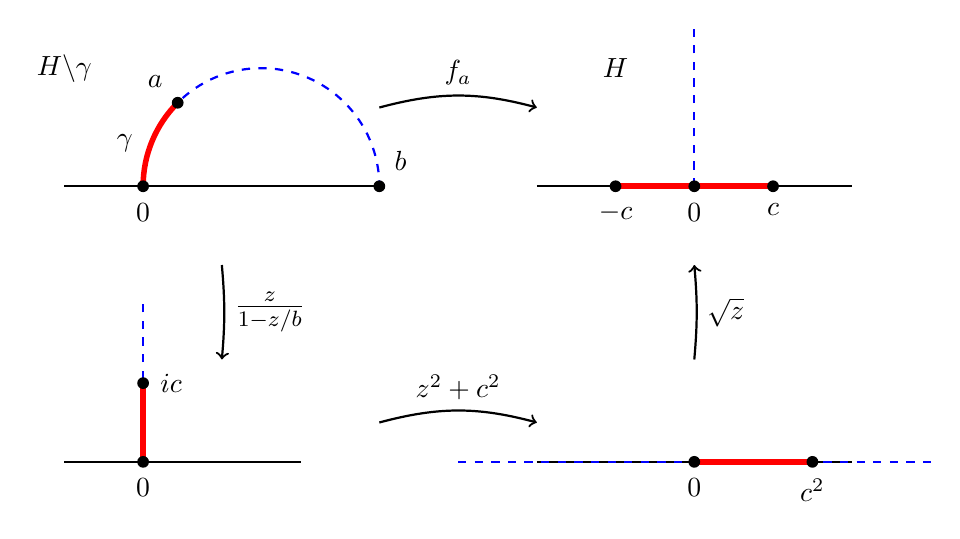
\begin{tikzpicture}[thick,
  dot/.style={fill=black,circle,inner sep=1.5pt}]

% Top left: H \ gamma
\begin{scope}[shift={(-4,2)}]
  \draw (-1,0) -- (3,0);
  \draw[dashed,blue] (0,0) arc[start angle=180,end angle=0,radius=1.5];
  \draw[red,line width=2pt] (0,0) arc[start angle=180,end angle=135,radius=1.5];
  \node[dot,label=below:$0$] at (0,0) {};
  \node[dot,label=above left:$a$] at ({-1.5*cos(45)+1.5},{1.5*sin(45)}) {};
  \node[dot,label=above right:$b$] at (3,0) {};
  \node[above left] at (0,0.3) {$\gamma$};
  \node at (-1,1.5) {$\mathbb{H}\backslash\gamma$};
\end{scope}

% Arrow from top left to top right
\draw[->] (-1,3) to[bend left=15] node[above] {$f_a$} (1,3);

% Top right: H
\begin{scope}[shift={(3,2)}]
  \draw (-2,0) -- (2,0);
  \draw[dashed,blue] (0,0) -- (0,2);
  \draw[red,line width=2pt] (-1,0) -- (1,0);
  \node[dot,label=below:$-c$] at (-1,0) {};
  \node[dot,label=below:$0$] at (0,0) {};
  \node[dot,label=below:$c$] at (1,0) {};
  \node at (-1,1.5) {$\mathbb{H}$};
\end{scope}

% Arrow from top left to bottom left
\draw[->] (-3,1) to[bend left=5] node[right, font=\large] {$\frac{z}{1-z/b}$} (-3,-0.2);

% Arrow from top right to bottom right
\draw[<-] (3,1) to[bend left=5] node[right] {$\sqrt{z}$} (3,-0.2);

% Bottom left
\begin{scope}[shift={(-4,-1.5)}]
  \draw (-1,0) -- (2,0);
  \draw[dashed,blue] (0,0) -- (0,2);
  \draw[red,line width=2pt] (0,0) -- (0,1);
  \node[dot,label=below:$0$] at (0,0) {};
  \node[dot,label=right:$ic$]at (0,1) {};
% \node[blue,right] at (0,0.5) {$ic$};
\end{scope}

% Arrow from bottom left to bottom right
\draw[->] (-1,-1) to[bend left=15] node[above] {$z^2+c^2$} (1,-1);

% Bottom right
\begin{scope}[shift={(3,-1.5)}]
  \draw (-2,0) -- (2,0);
  \draw[dashed,blue] (-3,0) -- (3,0);
  \draw[red,line width=2pt] (0,0) -- (1.5,0);
  \node[dot,label=below:$0$] at (0,0) {};
  \node[dot,label=below:$c^2$] at (1.5,0) {};
\end{scope}
\end{tikzpicture}

\bigskip

%\end{document}

Now suppose $z_0, z_1, ..., z_n$ are points arranged counterclockwise on a Jordan curve $\Gamma$ in the upper half plane. The geodesic algorithm basically iterates over the arcs from $z_i$ to $z_{i+1}$ and "unzips" them one by one using the map $f_{a_i}$ where $a_i$ is the image of $z_{i+1}$ under the composition of all previous maps.
The original geodesic algorithm proposed by Marshall and Rohde constructs a conformal map from the upper half plane to the region bounded by $\Gamma$, but it can be adapted to map from the unit disk as well via a Möbius transformation mapping the half plane to the unit disk and back first.

\begin{algorithm}
    \caption{Geodesic Zipper Algorithm}
    \begin{algorithmic}
    \STATE \textbf{Input:} Points $z_0, z_1, ..., z_n$ on a Jordan curve $\Gamma$ in the upper half plane.
    \STATE \textbf{Output:} $\psi$: conformal map from $\mathbb{H}$ to the region bounded by $\Gamma$ and its inverse $\psi^{-1}$.
    \STATE $\varphi_1(z) := i\sqrt{(z-z_1)/(z-z_0)}$
    \STATE $\zeta_2:= \varphi_1(z_2)$
    \STATE $\varphi_2(z) := f_{\zeta_2}(z)$
    \FOR{k in n}
        \STATE $\zeta_k := \varphi_{k-1} \circ \ldots \circ \varphi_1 (z_k)$
        \STATE $\varphi_k(z) := f_{\zeta_k}(z)$
    \ENDFOR
    \STATE Finally, $\zeta_{n+1} := \varphi_n \circ \ldots \circ \varphi_1 (z_{0})\in\R$ and $\varphi_{n+1}(z) := -(\frac{z}{1 - z/\zeta_{n+1}})^2$
    \STATE Then $\psi(z) := \varphi_1^{-1} \circ \varphi_2^{-1} \circ \ldots \circ \varphi_{n+1}^{-1}(z)$ and $\psi^{-1}(z) := \varphi_{n+1} \circ \ldots \circ \varphi_2 \circ \varphi_1 (z)$
    \end{algorithmic}
\end{algorithm}
\begin{flushleft}
\includegraphics[width=\textwidth]{zipper_geodesic.png}
\end{flushleft}

\subsubsection{The Slit Algorithm}
The above geodesic algorithm is only as accurate as the approximation of the boundary curve $\Gamma$ by circular arcs between the points $z_i$. A more accurate version is given by the slit algorithm, which uses straight line segments instead of circular arcs.
We therefore exchange the map $f_a$ for a map $g_a: \mathbb{H}\setminus L \to \mathbb{H}$ where $L$ is the line segment from $0$ to $a\in\mathbb{H}$. This map does not have a closed form expression, but can be computed numerically using Newton's method.

\subsubsection{The Zipper Algorithm}
The approximation of $\Gamma$ by circular arcs or straight line segments can be further improved by using circular arcs which meet $\Gamma$ tangentially at the points $z_i$. Each arc is determined by the points $z_i, z_{i+1}$ and $z_{i+2}$, hence we assume an even number of boundary points. 
The first arc is replaced by $$\varphi_1(z)=\sqrt{\frac{(z-z_2)(z_1-z_2)}{(z-z_0)(z_1-z_2)}}.$$ At each subsequent step that circular arc through $\zeta_k$ and $\zeta_{k+1}$ is mapped onto a straight line segment by a Möbius transform, and then the Slit Algorithm is applied to unzip that segment.
\red{This yields a sort of "quadratic approximation" of $\del\Omega$ instead of a linear one.}


\subsection{Wegmann's Method} \label{chap:WegmannMethod}
For smooth $\del\Omega$, Integral equations of the second kind can also be solved by Newton's method \cite{Wegmann1978_newtonverfahren}.
Given $\eta$ the differentiable parametrization of $\Gamma$ with $\dot\eta(s)\neq 0 \text{ } \forall s$, we construct the conformal mapping by iterated correction of an initial guess $S$ as follows: 
$$
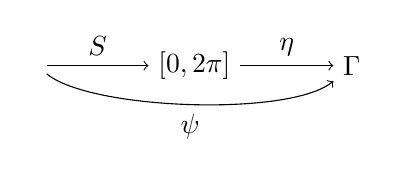
\begin{tikzpicture}[node distance=2cm, auto]
\node (A) {$\del\disk$};
\node(B) [right of=A] {$[0,2\pi]$};
\node (C) [right of=B] {$\Gamma$};
\draw[->](A) to node {$S$}(B);
\draw[->](B) to node {$\eta$}(C);
\draw[->, out = -40, in = -140, looseness = 0.5] (A) to node [below]{$\psi$}(C); % this should be a circular arrow under the diagram
\end{tikzpicture}
$$
%Assume a starting configuration of points $z_1, z_2, ..., z_N$ in $\disk$ and their images $\zeta_1, \zeta_2, ..., \zeta_N$ on $\Gamma$ such that $\psi(z_k)=\zeta_k$. 
Assume that the approximation for $\psi$ after $k$ steps be given by $\psi_k(\zeta)=\eta(S_k(\zeta))$. We improve the approximation by moving the points along their tangents towards the boundary curve, i.e. by finding a correction function $U_k:\del\disk\to[0,2\pi]$ such that
\begin{equation}\label{eq:h_k+1}
    \eta(S_k(\zeta))+U_k(\zeta)\dot\eta(S_k(\zeta)) = h_{k+1}(\zeta)
\end{equation}
where $h$ is analytic on $\overline\Omega$.
To uniquely solve for $U_k$ numerically, we fix a boundary point $z_0 \in\del\disk$ and its corresponding target parameter $s_0\in[0,2\pi]$ which defines the target point $\eta(s_0)=c_0\in\Gamma$. 
Note that since $h_{k+1}(z_0)$ lies on the tangent through $\eta(S_k(z_0))$ we cannot have $h_{k+1}(z_0)=c_0$ unless $\eta(S_k(z_0))=c_0$. Therefore we set
\begin{equation}
    U_k(z_0)=s_0-S_k(z_0).
\end{equation}
Note also that $h_{k+1}$ is an approximation of $\psi$ but it does not generally take values on $\Gamma$. We get an approximation for the parametrization $S$ by $$S_{k+1}(\zeta):= S_k(\zeta)+U_k(\zeta)$$ which can be understood as "new guess equals last guess plus some correction".

\subsubsection{Implementation}
Since we assume $\psi$ to map from the unit disk $\disk$, the integral equations can be explicitly solved by discretization and trigonometric interpolation:
Take $N=2n$ equidistant points $\zeta_k=e^{i\theta_k}$ on the boundary of the disk, where
$$\theta_k = \theta_0 + \frac{\pi k}{N}, \quad k\in[N-1]$$
and write the integrals in terms of their Fourier transform
\begin{equation}
    F(z)=\frac{1}{2\pi i}\int \frac{\sigma_n(\zeta)}{\zeta - z} d\zeta
\end{equation}
where $\sigma_n(\zeta_k)=\sum_{i=-n}^{n} c_k \zeta_k^i$. This can be computed fast ($\in\bigO(N\log N)$) via FFT.
% Then, given $\eta(s)$, $\dot\eta(s)$ and $\Theta(s):= arg(\dot\eta(s))$ in closed form, and given initial values $S_1(\zeta_k)$ the next iteration is computed as follows:


% \subsection{Shirokova's Method}
% \cite{Shirokova2014}

\subsection{Conjugate Function Method}
Hakula, Quach and Rasila \cite{Hakula_2013_conjugatefunctionmethod} presented a new method in 2010 which is based on numerical solution of the Laplace equation subject to Dirichlet-Neumann mexed-type boundary conditions by using $hp$-FEM.  
In their paper they construct the mapping starting from a quadrilateral, but it can be tweaked to map from the unit disk as well. 
"It is well known that one can express the modulus of a quadrilateral Q in terms of the solution of the Dirichlet-Neumann mixed boundary value problem \cite[p.431]{Henrici1986_vol3}."


\subsection{Amano's Method of Fundamental Solutions}
A potential theoretic formulation of the conformal mapping problem leads to a Fredholm integral equation of the first kind, known as Symm's integral equation, which has a kernel with logarithmic singularity. Unlike Fredholm integral equations of the second kind like Theodorsen's equation, where the singularity of the kernel creates numerical instabilities, Symm's equation is easily solvable by numerical methods \cite[p. 237]{Kythe1998_symmsintegralequation}. One of these is Amano's method.
Conceptually, a pair of conjugate harmonic functions are expressed by a complex logarithmic potential, and the mapping problems are reduced to singular Fredholm integral equations of the first kind. Gaier \cite{Gaier1964} mathematically studied Symm’s integral equation and proved the existence and uniqueness of the solution. These methods need $\bigO(N^3)$ operations if the boundary is discretized at N points. Henrici showed that complexity of $\bigO(N^2\log N)$ can be achieved by using FFTs \cite{Henrici1986_vol3}.

\begin{definition}
    In two dimensions, the Laplace equation has a fundamental solution of the form $log(r)$ where $r=|z-\zeta_k|$ is the modulus of the vector from any point $z$ on the region to the boundary point $\zeta_k$, $k\in N$. This function $log(|z-\zeta_k|)$ is called the \textbf{logarithmic potential}. 
\end{definition}
This is used in the so-called Charge Simulation Method which Amano's Method is based on.

\subsubsection{Algorithm}
The charge simulation method approximates the solution of the Laplace equation by a linear combination of fundamental solutions placed at so-called charge points outside the domain \cite{Amano1998_Amanosmethod} by 
\begin{equation}\label{eq:AmanosApproximation}
    g(z) = \sum_{k=1}^{N} Q_k log(|z-\zeta_k|),
\end{equation}
where $\zeta_1, \ldots, \zeta_N \notin\overline\Omega$ are called \textbf{charge points} and placed outside the domain (\red{their placement is an art in and of itself}). The unknown constants $Q_1, \ldots, Q_N$ are called \textbf{charges} and determined to satisfy the boundary condition at the \textbf{collocation points} $z_1, \ldots, z_N$ (fixed check points on the boundary $\del\Omega$).
Hence, $Q_k$ are found by plugging in the collocation points into the below \textbf{collocation condition} and solving the linear system:
\begin{equation} \label{eq:collocationCondition}
    \eta(z_i) = \sum_{k=1}^{N} Q_k log(|z_i-\zeta_k|), \quad i=1,2,...,N.
\end{equation}
Then the conformal map $\psi(z)=g(z)+ih(z)$ is constructed, where $h(z)$ is the harmonic conjugate of $g(z)$.
If the boundary is analytic, this method can be shown to have exponential accuracy i.e. exponentially small error in the number of collocation points \cite{Amano1998_Amanosmethod}.

%\cite{Sakakibara2019_AmanosMethod}

\subsection{Probabilistic Uniformization Method}
In 2007, Binder, Braverman ans Yampolsky proposed a method for finding a conformal map using a random walks solver to the general Dirichlet problem. They conjectured an upper bound of polynomial space and time for an algorithm with precision $\frac{1}{n}$ pixels (for explicitly given $\del\Omega$; quadratic if $\del\Omega$ is given only approximately, via a so-called \textit{oracle}, sort of a Dirac delta function). \cite{binder2007_computationalcomplexityriemannmapping}


\red{\subsection{Workarounds of Common Problems}
Finally, we discuss some known workarounds for common problems in conformal mapping algorithms.

\subsubsection{Osculation Methods}\label{chap:OsculationMethods}
Osculation methods are preliminary conformal maps that smooth the boundary curve $\Gamma$ of the domain $\Omega$ before applying a more accurate conformal mapping algorithm such as Theodorsen's method. 

\subsubsection{Crowding}\label{chap:crowding}
}




\subsection{Comparison}
We can directly rule out some of the options due to our project constraints: 
First we note that Schwarz-Christoffel only works on polygons and Theodorsen's method is restricted to star-shaped regions. Since we want to be able to work with more general shapes of $\Omega$, we have to disregard these two methods.

We refrain from using probabilistic methods due to their inherent randomness and the difficulty of guaranteeing a certain accuracy.
\red{Amano's Method of Fundamental Solutions seems good for fast point-evaluations of $\psi$ itself, but the derivative could be tricky due to $\psi$'s form.} Moreover, we cannot use our Fourier parametrization nor our mesh in this method, so it will probably not be the best choice for our specific problem. Note also that the accuracy and convergence of this method depend on the right choice of charge points, which poses another difficulty, especially given the generality of our target domain.
The Conjugate Function Method is very beautiful mathematically, but it relies only on $hp$-FEM for which there already are powerful libraries, so there would not be much value in half-assing an FEM solver given the scope of this thesis. 

On the one hand, the Zipper method seems very well implementable and robust, but there is a small caveat to be aware of for the efficient point evaluations. Since the Zipper method essentially constructs $\psi$ as a composition of many maps, the derivative is not straightforward to implement via a formula (chain rule). Also, trying a finite differences approach is slow and potentially numerically unstable, but there is hope in a technique called Forward Automatic Differentiation which is both exact and efficient \cite{wikipedia_autodiff}. 

On the other hand, the Alternating Projections Method uses the boundary parametrization in its Fourier series form.
The output of the discretized OAP is an interpolating polynomial, allowing for efficient point evaluations of $\psi$ and $D\psi$.
The AP Method converges linearly if the boundary parametrization is 3-Hölder and the initial approximation $U_0$ is sufficiently close to the actual boundary correspondence function (\ref{eq:boundaryCorrespondence}) \cite[p. 292]{Wegmann1989_alternating_projections}.
The Alternating Projections Method is one of the simplest and most robust methods for conformal mapping. However, it is not very accurate for reasonably sized grids, and converges very slowly for finer meshes \cite[p. 389]{Wegmann2005_num_methods_confmapping}.

Lastly, Wegmann's Method (\ref{chap:WegmannMethod}) uses the boundary parametrization and its derivative in form of Fourier coefficients as well as the tangent angle as inputs. 
The output of the algorithm is an analytic function constructed from trigonometric polynomials. This allows for efficient point evaluations of both $\psi$ and its derivative \cite{Wegmann1984_convergence_iterative_method}.
Convergence is quadratic for analytic boundaries (as is known for Newton methods) and superlinear ($\in\bigO(N^{1+\mu})$) for $\eta\in C^{2+\mu}$ but depends on a "good enough" initial guess for the correspondence function \cite{Wegmann1984_convergence_iterative_method}.
Discretizing the operator $K$ (\ref{operatorK_N}) using \red{Wittich's method} yields the operator $K_N$ which can be computed efficiently using FFT.

Wegmann also compared the accuracies of the AP, OAP, Theodorsen and Wegmann methods for the mapping from the disk to an inverted ellipse and found that OAP is most efficient for low accuracy and Newton methods are best for slower high accuracy calculations \cite[p. 415]{Wegmann2005_num_methods_confmapping}.
Note the computational costs of these last two methods are mainly determined by the FFTs and this parameter is dependent on the number of grid points.

Hence, Zipper, OAP and Wegmann's methods seem suitable for our problem, \red{but Wegmann's Method is more accurate with faster convergence while OAP is easier to implement. COMPARISON TABLE HERE}

\bigskip


\iffalse
\begin{sidewaystable}[!p]
\caption{Overview Table}
\centering
\small
\resizebox{\textwidth}{!}{%
    \begin{tabular}{|l|l|l|l|l|l|l|l|}
    \hline
    Algorithm & $\Omega$ shape & Runtime & Space & Input & Output & Advantages & Disadvantages \\
    \hline
    Alternating projections& shape & Runtime & Space & Input & Output & Advantages & Disadvantages\\
    \hline
    Zipper &shape & Runtime & Space & Input & Output & Advantages & Disadvantages \\
    \hline
    Theodorsen & star-shaped & Runtime & Space & Input & Output & Advantages & Disadvantages \\
    \hline
    Schwarz-Christoffel & polygon  & Runtime & Space & Input & Output & corner-handling & disadvantages\\
    \hline
    Niethammer &shape & Runtime & Space & linear system of equations & Output & Advantages & Disadvantages\\
    \hline
    Wegmann & shape & Runtime & Space & non-linear Theodorsen Equation & Output & Advantages & Disadvantages \\
    \hline
    Conjugate fct & shape & Runtime & Space & Input & Output & Advantages & Disadvantages \\
    \hline
    Spare row & shape & Runtime & Space & Input & Output & Advantages & Disadvantages\\
    \hline
    \end{tabular}%
}
\end{sidewaystable}
\fi